\chapter{実装}
\section{概要}
\SysName は、ハードウェアとして三角法を用いた光学式距離センサ10個を一列に並べたセンサアレイと、センサから取得した値の処理と値を元に座標を計算するソフトウェアからなる。
\section{ハードウェア}
距離センサはSHARP GP2Y0E03\footnote{http://www.sharp.co.jp/products/device/lineup/selection/opto/haca/diagram2.html}を使用した。この距離センサは三角測量の原理を用い、対象までの距離を計測する。本センサの値の取得には、Arduino MEGA 2560を用いる。距離センサとは\iic を用いて接続を行う。個々のセンサは、スレーブアドレスが初期値(0x40)で統一されているために、アプリケーションノート\footnote{http://www.sharp.co.jp/products/device/doc/opto/gp2y0e02\_03\_appl\_j.pdf}に記載されているe-fuseプログラミングの手順で、スレーブアドレスの変更を行なっている。これにより、10個の距離センサを2本の信号線で制御する。
接続した距離センサは1列に並べる。\SysName では、30cmのプラスティック製の定規を用意し、両面テープでセンサ本体を固定し、配線類をセロハンテープで固定した。\refImg{ig1}は実際に製作したプロトタイプの1つである。\refImg{ig1}ではセンサごとの間隔は約11\si{mm}としている。
\begin{figure}[htbp]
	\begin{center}
		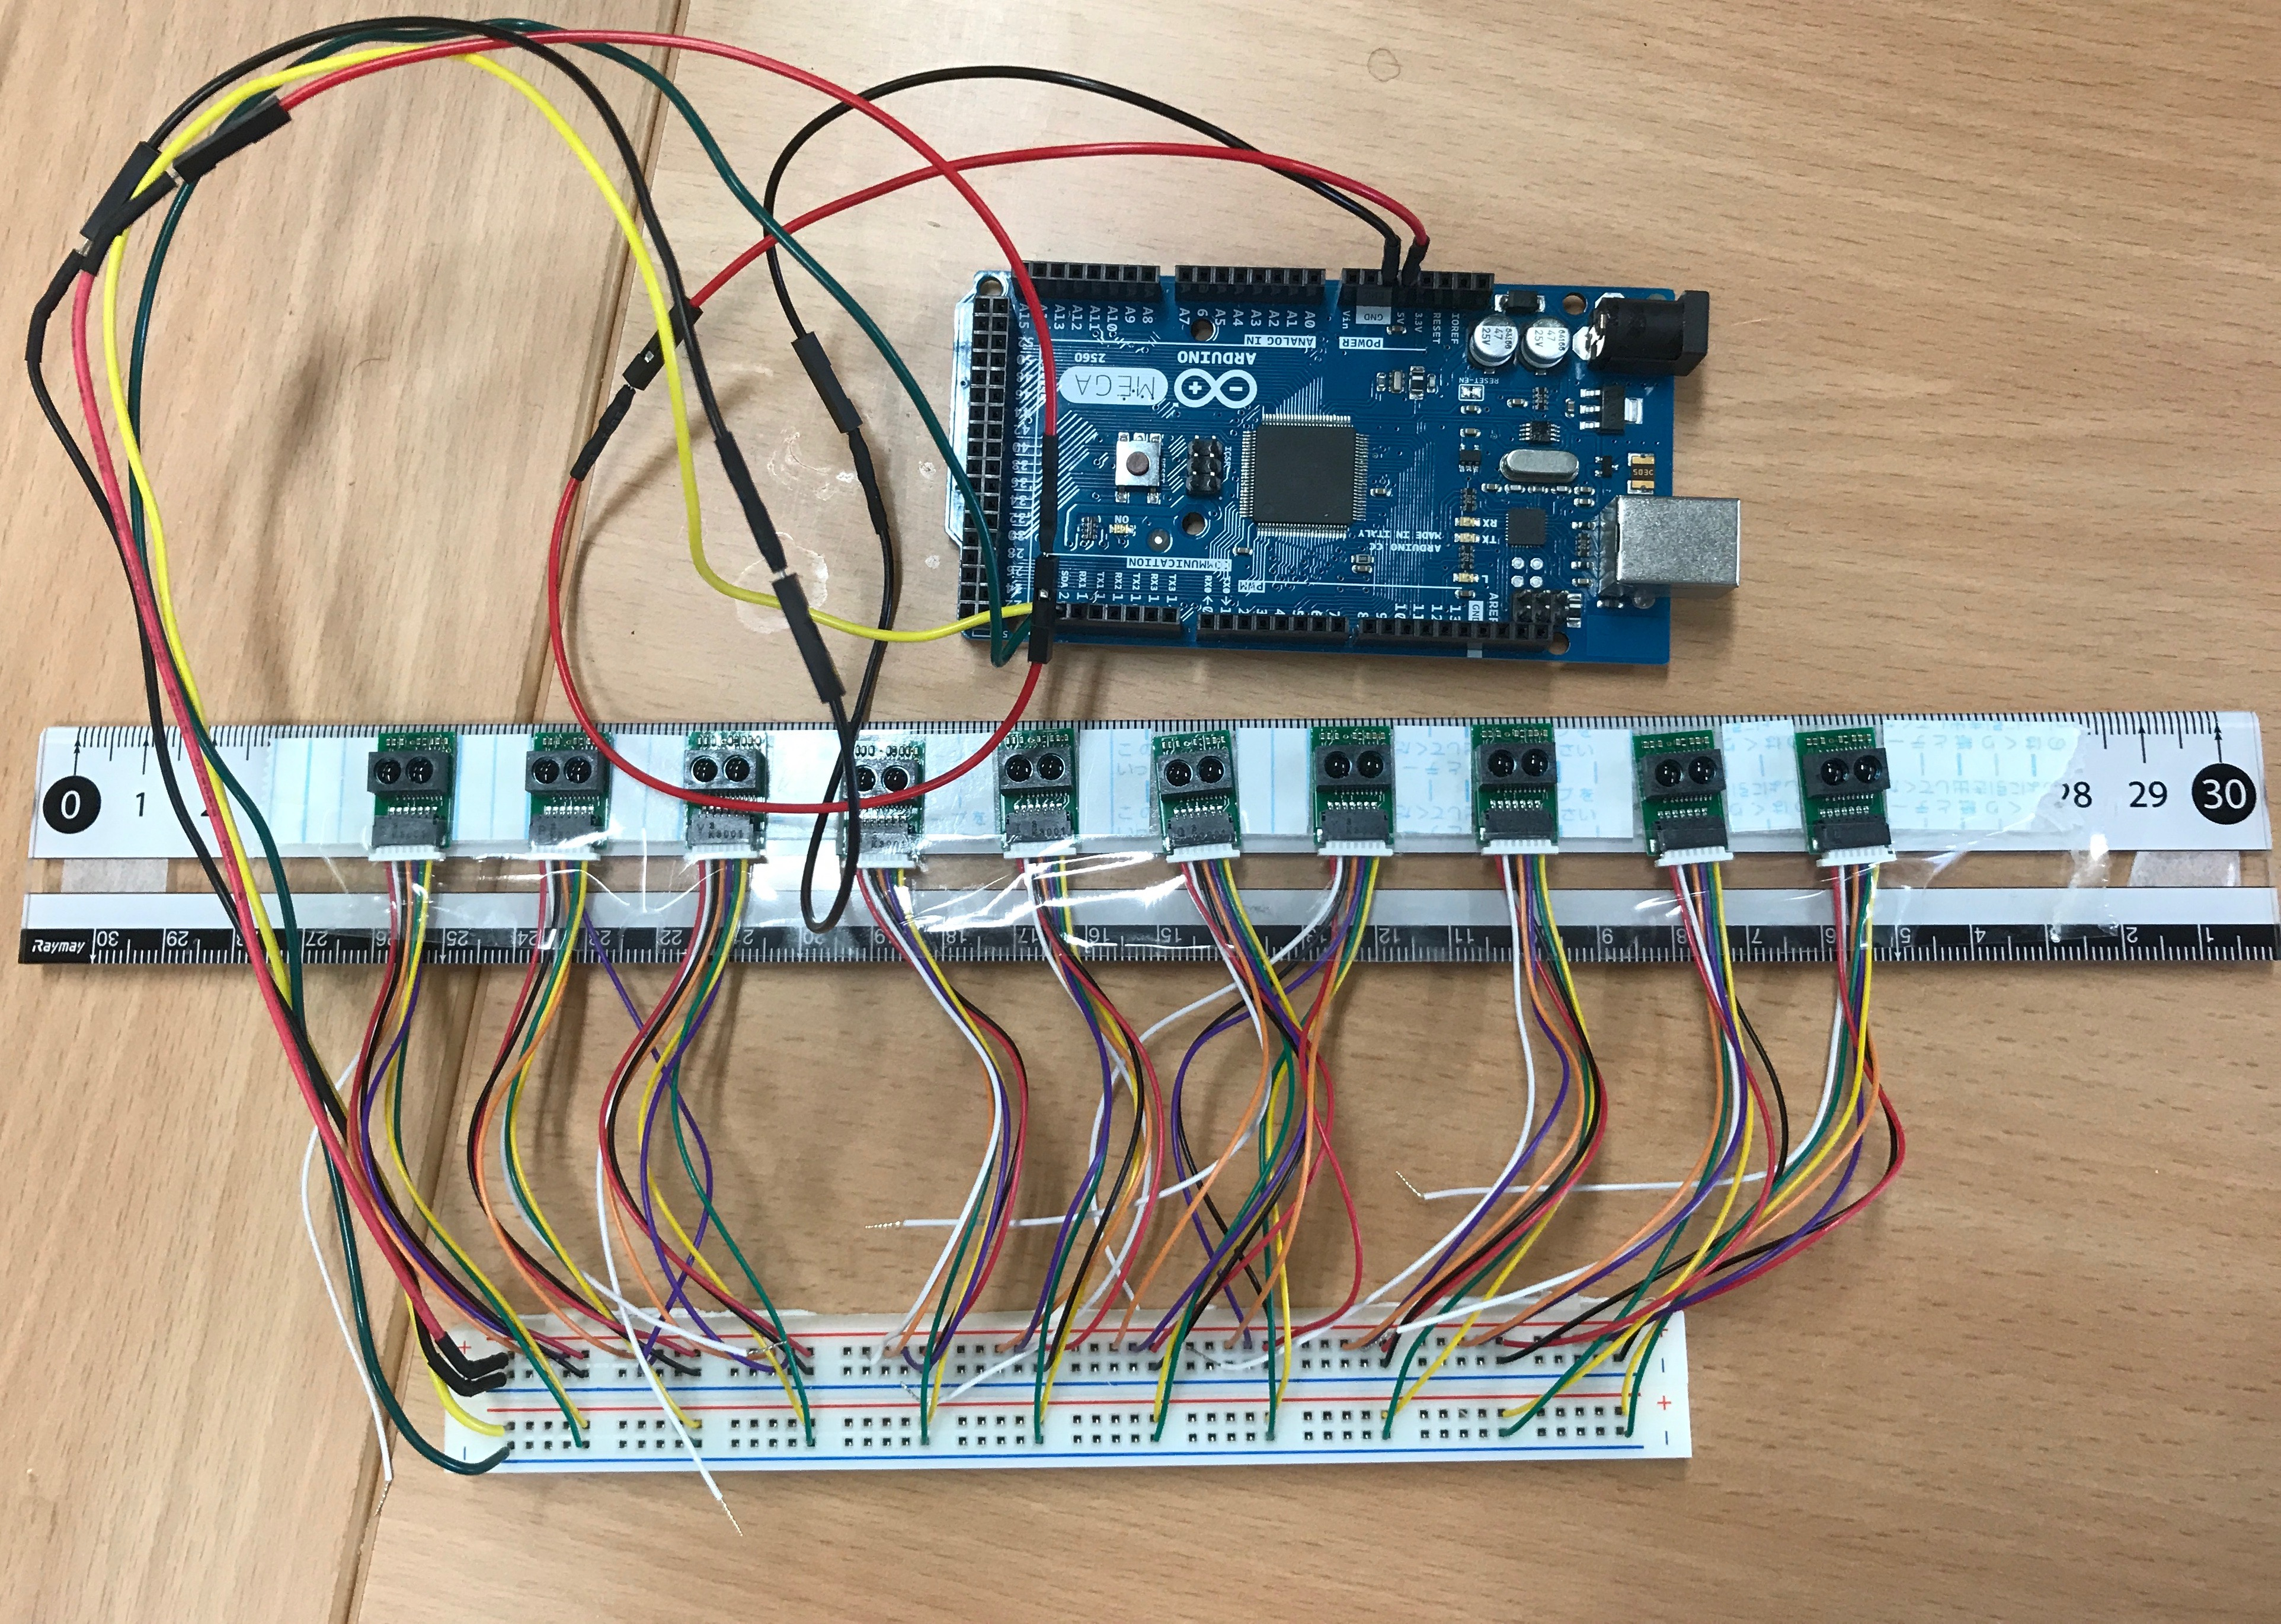
\includegraphics[width = 90mm]{./img/IMG_1794.jpg}
	\end{center}
	\caption{\fixme{プロトタイプその1}}
	\label{img:ig1}
\end{figure}
\section{ソフトウェア} 


